%%%%%%%%%%%%%%%%%%%%%%%% ExtendedAbstract.tex %%%%%%%%%%%%%%%%%%%%%%%%
%                                                                    %
%  Template for the 10-page extended abstract to be submitted for    %
%  the MSc degree conferral at Instituto Superior Tecnico.           %
%                                                                    %
%  Author:                                                           %
%                                                                    %
%       Andre C. Marta                                               %
%       Area Cientifica de Mecanica Aplicada e Aeroespacial          %
%       Departamento de Engenharia Mecanica                          %
%       Instituto Superior Tecnico                                   %
%       Av. Rovisco Pais                                             %
%       1049-001 Lisboa                                              %
%       Portugal                                                     %
%       Tel: +351 21 841 9466                                        %
%                        3466 (extension)                            %
%       Email: andre.marta@ist.utl.pt                                %
%                                                                    %
%  Created:       Dec  2, 2011                                       %
%  Last Modified: Dec 27, 2011                                       %
%%%%%%%%%%%%%%%%%%%%%%%%%%%%%%%%%%%%%%%%%%%%%%%%%%%%%%%%%%%%%%%%%%%%%%
% This document uses the LaTeX class file "article.cls"              %
%%%%%%%%%%%%%%%%%%%%%%%%%%%%%%%%%%%%%%%%%%%%%%%%%%%%%%%%%%%%%%%%%%%%%%
\documentclass[10pt,a4paper,twocolumn]{article}

%%%%%%%%%%%%%%%%%%%%%%%%%%%%%%%%%%%%%%%%%%%%%%%%%%%%%%%%%%%%%%%%%%%%%%
% Document preamble
%%%%%%%%%%%%%%%%%%%%%%%%%%%%%%%%%%%%%%%%%%%%%%%%%%%%%%%%%%%%%%%%%%%%%%

%% Builds upon the graphics  package, providing a key-value interface
%% for optional arguments to the \includegraphics command that go far
%% beyone what the graphics package offers.
%% http://www.ctan.org/tex-archive/help/Catalogue/entries/graphicx.html
%% if you use PostScript figures in your article
%% use the graphics package for simple commands
%% \usepackage{graphics}
%% or use the graphicx package for more complicated commands
%% \usepackage{graphicx}
%% or use the epsfig package if you prefer to use the old commands
%% \usepackage{epsfig}
\usepackage{graphicx} % Enhanced LaTeX Graphics

% Multiple figures
\usepackage{subfigure} % subcaptions for subfigures
\usepackage{subfigmat} % matrices of similar subfigures

% Declaring new column types
% 'dcolumn' package defines D to be a column specifier with
% three arguments: D{<sep.tex>}{<sep.dvi>}{<decimal places>}
%                  D{<sep.tex>}{<sep.dvi>}{<left digit places>.<right digit places>}
\usepackage{dcolumn}           % decimal-aligned tabular math columns
% d takes a single argument specifying the number of decimal places, e.g., d{2}
% or the number of digits to the left and right of the seperator, e.g., d{3.2}
\newcolumntype{.}   {D{.}{.}{-1}} % column alignedd on the point separator '.'
\newcolumntype{d}[1]{D{.}{.}{#1}} % column centered on the point separator '.'
\newcolumntype{e}   {D{E}{E}{-1}} % column centered on the exponent 'E'
\newcolumntype{E}[1]{D{E}{E}{#1}} % column centered on the exponent 'E'

%% American Mathematical Society (AMS) plain Tex macros
%%
%% The amsmath package is the principal package in the AMS-LaTeX distribution
%% http://www.ctan.org/tex-archive/help/Catalogue/entries/amsmath.html
\usepackage{amsmath}
%%
%% The amsfonts package provides extended TeX fonts
%% http://www.ctan.org/tex-archive/help/Catalogue/entries/amsfonts.html
\usepackage{amsfonts}
%% The amssymb package provides various useful mathematical symbols
\usepackage{amssymb}
%%
%% The amsthm package provides extended theorem environments
%% http://www.ctan.org/tex-archive/help/Catalogue/entries/amsthm.html
\usepackage{amsthm}

%% Improves the interface for defining floating objects such as figures and tables.
%% The package also provides the H float modifier option of the obsolete here package.
%% http://www.ctan.org/tex-archive/help/Catalogue/entries/float.html
\usepackage{float}

%% Control sectional headers. 
%% http://www.ctan.org/tex-archive/help/Catalogue/entries/sectsty.html
\usepackage{sectsty}
%%
%% Redefine the font size of the 'section' and 'subsection' headings
\newcommand{\myFontSize}{\fontsize{10}{0}\selectfont}
\sectionfont{\myFontSize}       % 10pt, Bold face (default)
\subsectionfont{\rm\myFontSize} % 10pt, Plain face

%% Select alternative section titles.
%% http://www.ctan.org/tex-archive/help/Catalogue/entries/titlesec.html
\usepackage{titlesec}
%%
%% Left indent, before and after spacing
%% (The starred version kills the indentation of the paragraph following the title)
\titlespacing*{\section}{0pt}{10pt}{0pt}
\titlespacing*{\subsection}{0pt}{10pt}{0pt}

%% Section numbers with trailing dots. 
%% http://www.ctan.org/tex-archive/help/Catalogue/entries/secdot.html
\usepackage{secdot}
%%
%% Also put a dot after the subsection number
\sectiondot{subsection}
%% Set a space between dot and heading text
\sectionpunct{section}{. }    % By default, \sectiondot places a \quad
\sectionpunct{subsection}{. } % after the number

% These are exact settings for a A4 page with top margin of
% 25 mm, bottom margin of 30 mm, left and right margins of 25 mm,
% printable area 242 X 160 mm.

\setlength{\topmargin}{-10.4mm}
\setlength{\headheight}{0.0mm}
\setlength{\headsep}{10.0mm}
\setlength{\textwidth}{160mm}
\setlength{\textheight}{242mm}
\setlength{\oddsidemargin}{0mm}
\setlength{\evensidemargin}{0mm}
\setlength{\marginparwidth}{0mm}
\setlength{\marginparsep}{0mm}

% New command to refer to equations as Eq.(1),Eq.(2),...
\newcommand{\eqnref}[1]{Eq.(\ref{#1})}

%%%%%%%%%%%%%%%%%%%%%%%%%%%%%%%%%%%%%%%%%%%%%%%%%%%%%%%%%%%%%%%%%%%%%%%%%%%%%%%%%%%%%%%%
% Title, authors and addresses

\title{Linux-capable RISC-V CPU for IOb-SoC}
\date{November 2022}
\author{Pedro Nuno de Melo Antunes \\ pedronmantunes@tecnico.ulisboa.pt \\ \\ Instituto Superior T\'{e}cnico, Lisboa, Portugal}

%%%%%%%%%%%%%%%%%%%%%%%%%%%%%%%%%%%%%%%%%%%%%%%%%%%%%%%%%%%%%%%%%%%%%%%%%%%%%%%%%%%%%%%%
\begin{document}

% Begin one column section for title and abstract
%
% http://www.faqs.org/faqs/de-tex-faq/part5/
\twocolumn[
\begin{@twocolumnfalse}
\maketitle

%%%%%%%%%%%%%%%%%%%%%%%%%%%%%%%%%%%%%%%%%%%%%%%%%%%%%%%%%%%%%%%%%%%%%%
% ABSTRACT & KEYWORDS
%%%%%%%%%%%%%%%%%%%%%%%%%%%%%%%%%%%%%%%%%%%%%%%%%%%%%%%%%%%%%%%%%%%%%%
%%%%%%%%%%%%%%%%%%%%%%%%%%%%%%%%%%%%%%%%%%%%%%%%%%%%%%%%%%%%%%%%%%%%%%
%     File: ExtendedAbstract_abstr.tex                               %
%     Tex Master: ExtendedAbstract.tex                               %
%                                                                    %
%     Author: Andre Calado Marta                                     %
%     Last modified : 2 Dez 2011                                     %
%%%%%%%%%%%%%%%%%%%%%%%%%%%%%%%%%%%%%%%%%%%%%%%%%%%%%%%%%%%%%%%%%%%%%%
% The abstract of should have less than 500 words.
% The keywords should be typed here (three to five keywords).
%%%%%%%%%%%%%%%%%%%%%%%%%%%%%%%%%%%%%%%%%%%%%%%%%%%%%%%%%%%%%%%%%%%%%%

%%
%% Abstract
%%
\begin{abstract}

Place abstract here.
%
No paragraph breaks.
\\
%%
%% Keywords (max 5)
%%
\noindent{{\bf Keywords:}} Keyword1, Keyword2, Keyword3, Keyword4, Keyword5 \\

\end{abstract}



% End one column section (begin default two columns)
\end{@twocolumnfalse}
]
%%%%%%%%%%%%%%%%%%%%%%%%%%%%%%%%%%%%%%%%%%%%%%%%%%%%%%%%%%%%%%%%%%%%%%
% INTRODUCTION
%%%%%%%%%%%%%%%%%%%%%%%%%%%%%%%%%%%%%%%%%%%%%%%%%%%%%%%%%%%%%%%%%%%%%%
%%%%%%%%%%%%%%%%%%%%%%%%%%%%%%%%%%%%%%%%%%%%%%%%%%%%%%%%%%%%%%%%%%%%%%
%     File: ExtendedAbstract_intro.tex                               %
%     Tex Master: ExtendedAbstract.tex                               %
%                                                                    %
%     Author: Andre Calado Marta                                     %
%     Last modified : 27 Dez 2011                                    %
%%%%%%%%%%%%%%%%%%%%%%%%%%%%%%%%%%%%%%%%%%%%%%%%%%%%%%%%%%%%%%%%%%%%%%
% State the objectives of the work and provide an adequate background,
% avoiding a detailed literature survey or a summary of the results.
%%%%%%%%%%%%%%%%%%%%%%%%%%%%%%%%%%%%%%%%%%%%%%%%%%%%%%%%%%%%%%%%%%%%%%

\section{Introduction}
\label{sec:intro}

\subsection{Motivation}

The availability of fully open-source systems capable of executing an Operating System (OS) is limited. For a long time, the Linux kernel~\cite{torvalds1997linux} and the open-source software built around it allowed developers
to implement a fully open-source Linux OS on their closed-source hardware devices. However, the scarcity of open-source hardware complicated the development of fully open-source systems. With the appearance of \textit{RISC-V}~\cite{asanovic2014instruction}, open-source hardware availability started growing. Developing a \textit{RISC-V} System on a chip (SoC) capable of executing a Linux OS would allow researchers to access a fully open-source system executing an OS. Having a Linux OS running in an SoC would allow developers to create new applications to run in that SoC without worrying about its hardware components. The Linux community is significant, and researchers are used to working with the Linux kernel. Therefore, the requirement for an SoC capable of running Linux is high. 

A Linux OS allows using many features unavailable in bare-metal applications. When developers create a bare-metal application, they must be aware of the SoC hardware and are limited in terms of functionalities. Similarly, if developers were to create an application using Real-Time Operating Systems (RTOS), for example, \textit{freeRTOS}~\cite{barry2008freertos}, they would have access to features such as a scheduler, events, threads, semaphores and message boxes. However, a Linux OS provides those and more functionalities. A Linux OS implements memory management and protection mechanisms, allows the execution of multiple applications simultaneously, supports multiple network adapters, and can interact with the user through a terminal. A Linux OS is also more secure than bare-metal or RTOS applications since it limits the user application's access to the machine resources, preventing misuse or damage.

What most motivates the development of a \textit{RISC-V} SoC capable of running a Linux OS is its advantages for future development. Such as creating hardware accelerators which work with a Linux OS and integrating them with the SoC the author developed to test in a real-world application.

\subsection{Objectives and Deliveries}

This dissertation work aims to develop an open-source SoC and execute a minimal Linux OS on it. The author will adapt the existing \textit{IOb-SoC}~\cite{iob_soc} to create an SoC that supports a Linux OS. \textit{IOb-SoC} is a modular open-source \textit{RISC-V} SoC that allows researchers to develop their own SoC. The IObundle developers use \textit{Verilog}~\cite{thomas2008verilog} to describe \textit{IOb-SoC} and peripherals hardware.

The author had first to swap the current CPU used in \textit{IOb-SoC}. The problem with the current CPU is that it cannot run an OS, only bare-metal applications. Therefore, \textit{IOb-SoC-Linux} contains a 32-bit \textit{RISC-V} CPU capable of running Linux. Then, since the \textit{IOb-SoC} does not support interrupts, the author had to create and integrate into \textit{IOb-SoC-Linux} the hardware needed to generate interrupts in a \textit{RISC-V} SoC. Lastly, the author had to ensure the Linux OS supported the UART used in the\textit{IOb-SoC-Linux}. Since Linux does not support the \textit{IOb-SoC} UART, the author integrated a UART16550 in \textit{IOb-SoC-Linux}.

Four major software components comprise a Linux OS. Those software components are the Linux kernel, the bootloader firmware, the root file system (rootfs) and a Device Tree Blob (DTB). The author had to build those software components to run a Linux OS on the \textit{IOb-SoC-Linux}. On power-on, the \textit{IOb-SoC-Linux} transfers the Linux OS software binary files onto the board where it runs, and the Linux OS will boot. After the OS boots, the user can run custom applications and take advantage of the Linux OS. The author also automated and documented the process of generating and deploying the Linux image to \textit{IOb-SoC-Linux} so that, after this work, creating new images with different characteristics will be straightforward.

Finally, the system must be fully verified both on simulation and running on an FPGA board. The \textit{IOb-SoC} needed a fast \textit{Verilog} simulator to verify the Linux OS execution. Therefore, the author developed a simulation testbench using the free-of-charge and open-source \textit{Verilator}~\cite{snyder2010verilator} simulator.


%%%%%%%%%%%%%%%%%%%%%%%%%%%%%%%%%%%%%%%%%%%%%%%%%%%%%%%%%%%%%%%%%%%%%%
% BACKGROUND
%%%%%%%%%%%%%%%%%%%%%%%%%%%%%%%%%%%%%%%%%%%%%%%%%%%%%%%%%%%%%%%%%%%%%%
%%%%%%%%%%%%%%%%%%%%%%%%%%%%%%%%%%%%%%%%%%%%%%%%%%%%%%%%%%%%%%%%%%%%%%
%     File: ExtendedAbstract_backg.tex                               %
%     Tex Master: ExtendedAbstract.tex                               %
%                                                                    %
%     Author: Andre Calado Marta                                     %
%     Last modified : 27 Dez 2011                                    %
%%%%%%%%%%%%%%%%%%%%%%%%%%%%%%%%%%%%%%%%%%%%%%%%%%%%%%%%%%%%%%%%%%%%%%
% A Theory section should extend, not repeat, the background to the
% article already dealt with in the Introduction and lay the
% foundation for further work.
%%%%%%%%%%%%%%%%%%%%%%%%%%%%%%%%%%%%%%%%%%%%%%%%%%%%%%%%%%%%%%%%%%%%%%

\section{Important Hardware and Software Concepts}
\label{sec:must_have_concepts}

This section discusses topics that help understand the technological developments along this thesis project. The developments involve both hardware and software components. As such, there are hardware and software concepts that are important to have before discussing the following chapters.

%%%%%%%%%%%%%%%%%%%%%%%%%%%%%%%%%%%%%%%%%%%%%%%%%%%%%%%%%%%%%%%%%%%%%%
\subsection{The \textit{IOb-SoC} platform}

The \textit{IOb-SoC}~\cite{iob_soc} is a System on a chip (SoC) template that eases the creation of a new SoC. The IObSoC provides a base \textit{Verilog}~\cite{thomas2008verilog} hardware design equipped with an open-source RISC-V processor, an internal SRAM memory subsystem, a UART, and an optional interface to external memory. If the external memory interface is selected, the \textit{IOb-SoC} will include an instruction L1 cache, a data L1 cache and a shared L2 cache. The L2 cache communicates with a third-party memory controller IP (typically a DDR controller) using an \textit{AXI4}~\cite{tidala2018high} master bus.

Figure \ref{fig:bd_original} represents a sketch of the SoC design. This design is valid at the start of this project. During the hardware development the \textit{IOb-SoC} original template suffered a few alterations.

\begin{figure}[!ht]
  \centering
  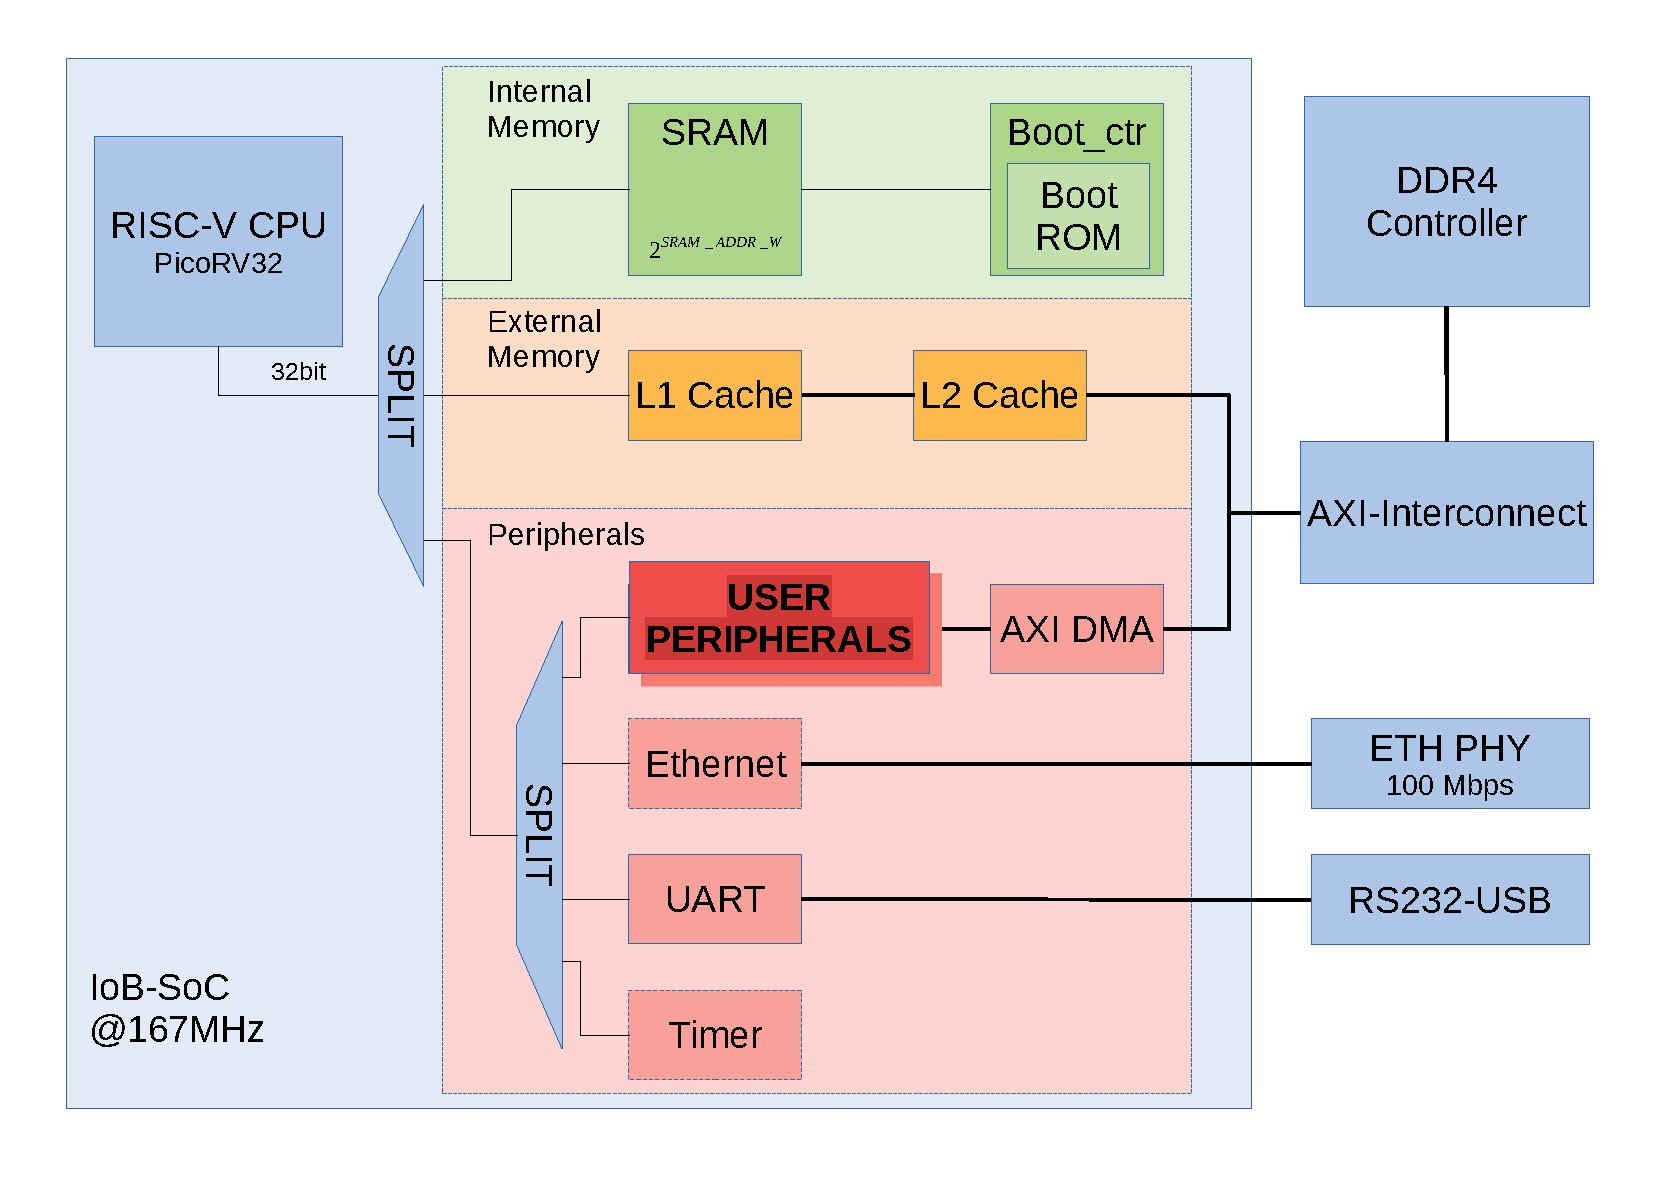
\includegraphics[width=\linewidth]{../images/bd_original.pdf}
  \caption{\textit{IOb-SoC} sketch.}
  \label{fig:bd_original}
\end{figure}

\textit{IOb-SoC} currently supports two FPGA board models: the \textit{Xilinx Kintex UltraScale KU040 Development Board} and the \textit{Cyclone V GT FPGA Development Kit}.

The main \textbf{\textit{Makefile}} in \textit{IOb-SoC} is located at the \textit{IOb-SoC} root directory. The main \textit{Makefile} contains targets that call other \textit{Makefiles} and sets the values for the default frequency, baud rate, FPGA board used and simulator used. The \textit{Makefiles} the main one can call are at the \textit{IOb-SoC} FPA boards, simulators, firmware, "PC" emulation or documentation directory. Each directory in \textit{IOb-SoC} contains a "*.mk" file which holds "make" variables and targets that complement the \textit{Makefiles}. The \textit{IOb-SoC} \textit{Makefiles} can include only the "*.mk" they need.

A \textit{IOb-SoC} \textbf{peripheral} should have the following "*.mk" files to integrate it into \textit{IOb-SoC}:
\begin{itemize}
    \item the "PERIPHERAL\_REPO/hardware/hard-ware.mk" so the user can add the peripheral hardware modules to the SoC.
    \item the "PERIPHERAL\_REPO/software/embe-dded/embedded.mk" allows the user to use the peripheral firmware drivers.
    \item the "PERIPHERAL\_REPO/software/pc-emul/pc-emul.mk" permits emulating the peripheral behaviour in the user's computer.
\end{itemize}

The \textit{IOb-SoC} \textbf{request bus} comprises a valid bit, an address signal, a data signal and a strobe signal. The hardware sets the valid bit to '1' when it wants to execute a request and has already defined the other signals. The address signal indicates the register that the request is targeting. Figure \ref{fig:req_bus} shows how the \textit{IOb-SoC} distributes the signals in the request bus. Furthermore, figure \ref{fig:req_bus} also represents the bits equivalent to each signal when the address width and data width are 32 bits. The address and data width in \textit{IOb-SoC} are 32-bit by default.

\begin{figure}[!ht]
    \centering
    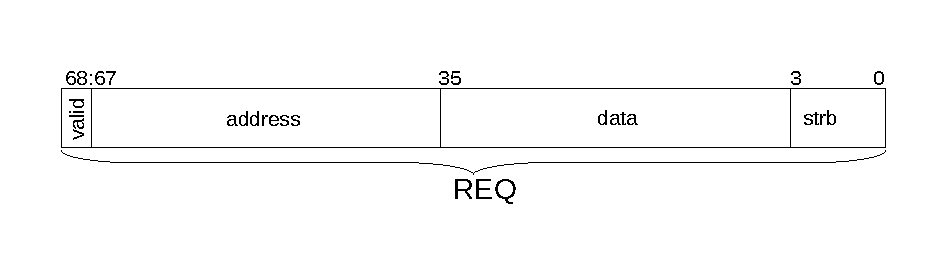
\includegraphics[width=\linewidth]{../images/req_bus.pdf}
    \caption{Request bus with address and data width equal to 32 bits.}
    \label{fig:req_bus}
\end{figure}

The \textit{IOb-SoC} \textbf{response bus} contains a ready bit and a data signal. The hardware sets the ready signal to high when the component that made the request can receive the response. The data signal is the response data to the request made. For example, if the CPU wants to read the value in a register at address "x", the data in the response bus will be the data on register "x". Figure \ref{fig:resp_bus} shows how the request signal is composed when the address and data width are 32 bits.

\begin{figure}[!ht]
    \centering
    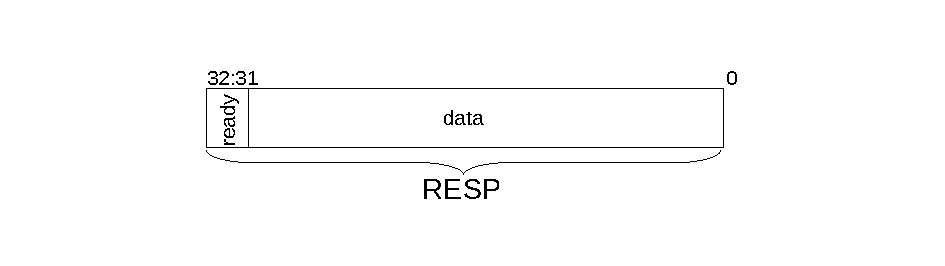
\includegraphics[width=\linewidth]{../images/resp_bus.pdf}
    \caption{Response bus with address and data width equal to 32 bits.}
    \label{fig:resp_bus}
\end{figure}

The \textbf{\textit{iob-split}} is simply a configurable demultiplexer (DEMUX). The developer can configure it when he instantiates the \textit{iob-split} hardware module. The developer can change the size of the DEMUX and the selection bits through N\_SLAVES and P\_SLAVES, respectively. N\_SLAVES corresponds to the number of slaves. Developers can also interpret N\_SLAVES as the number of the DEMUX outputs. P\_SLAVES indicates the slave select word most significant bit (msb) position. In other words, P\_SLAVES is the position of the msb of the DEMUX selection bits. Equation \ref{eq:number_bits} calculates the number of the selection bits.

\begin{equation}
    \label{eq:number_bits}
    Nb = log_2(N\_SLAVES)+(log_2(N\_SLAVES)==0)
\end{equation}

The \textbf{\textit{iob-merge}} works similar to the \textit{iob-split} but instead of being a DEMUX it is a configurable multiplexer (MUX). Meaning that instead of having multiple outputs and one input, it has multiple inputs and one output. N\_SLAVES indicates the number of inputs, and P\_SLAVES chooses the selection bits.

The \textit{IOb-SoC} \textbf{bootloader} is the first firmware to run on the SoC. Figure \ref{fig:boot_flow} represents a flow chart of the bootloader firmware behaviour.

\begin{figure}[!h]
    \centering
    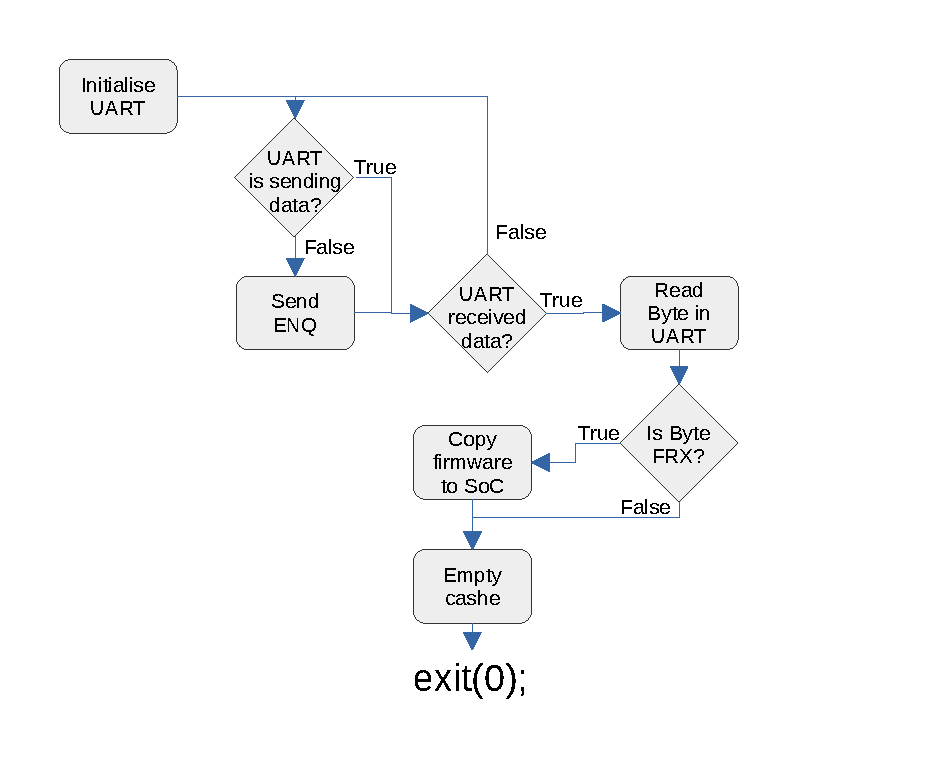
\includegraphics[width=\linewidth]{../images/boot_flow.pdf}
    \caption{Bootloader firmware flow chart.}
    \label{fig:boot_flow}
\end{figure}

%%%%%%%%%%%%%%%%%%%%%%%%%%%%%%%%%%%%%%%%%%%%%%%%%%%%%%%%%%%%%%%%%%%%%%
\subsection{\textit{RISC-V}}

\textit{RISC-V}~\cite{asanovic2014instruction} is a free-to-use, open-source RISC Instruction set architecture (ISA). The \textit{RISC-V} ISA defines the instructions which a \textit{RISC-V} compatible CPU can interpret. Those instructions represent the software written in C, Python, or any other programming language to be executed by the CPU.

The \textit{RISC-V} ISA is divided in two main volumes. The "RISC-V Instruction Set Manual Volume I"~\cite{riscv_unprivilege} contains the specification for the \textbf{unprivileged} instructions. The unprivileged instructions are instructions that do not need any special permission to execute. The "RISC-V Instruction Set Manual Volume II"~\cite{riscv_privilege} defines the \textit{RISC-V} \textbf{privilege} levels and the instructions that take advantage of them. Table \ref{tab:riscv_privilege_levels} shows the privilege levels currently defined in the \textit{RISC-V} specification. Developers must implement all three privilege levels to run a Unix-like OS.

\begin{table}[!ht]
  \centering
  \begin{tabular}{|l|l|l|l|}
  \hline
  \textbf{Level} & \textbf{Name}    & \textbf{Abbreviation} \\ \hline
  0              & User/Application & U                     \\ \hline
  1              & Supervisor       & S                     \\ \hline
  2              & Reserved         &                       \\ \hline
  3              & Machine          & M                     \\ \hline
  \end{tabular}
  \caption{\textit{RISC-V} privilege levels.}
  \label{tab:riscv_privilege_levels}
\end{table}

The \textit{RISC-V} \textbf{CLINT} specification~\cite{clint_riscv_spec} describes the hardware registers of a Core-local Interrupt Controller (CLINT) compatible with \textit{RISC-V} platforms. The hardware uses the CLINT to generate the inter-processor software and timer interrupts.

The \textit{RISC-V} systems use the Platform-Level Interrupt Controller (\textbf{PLIC}) hardware to gather various device interrupts and have only one external interrupt line per \textit{RISC-V} Hart context. A PLIC that claims to be a PLIC-Compliant standard PLIC has to follow the \textit{RISC-V} PLIC specification~\cite{plic_riscv_spec}.

In the \textit{RISC-V} Platform Specification~\cite{riscv_platform_specification} it is defined that every embedded OS is required to have a UART port implementation that is register-compatible with the industry standard \textbf{\textit{UART16550}}. The \textit{UART16550} already existed for a long time and developers often use it to connect to an RS-232 interface.

The Supervisor Binary Interface (\textbf{SBI}) specification~\cite{sbi_riscv_spec} defines an abstraction for platform-specific functionalities. Figure \ref{fig:riscv_sbi} illustrates the purpose of the SBI in a system executing an OS like the one the author is going to develop in this thesis.

\begin{figure}[!h]
    \centering
    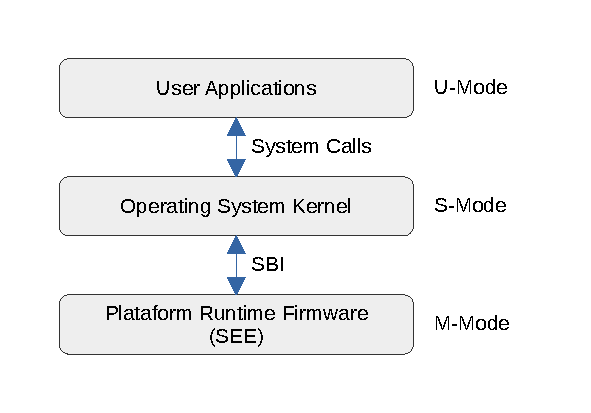
\includegraphics[width=0.8\linewidth]{../images/riscv_sbi.pdf}
    \caption{\textit{RISC-V} system running an OS.}
    \label{fig:riscv_sbi}
\end{figure}

\textbf{\textit{OpenSBI}} is the recommended interface between a platform-specific firmware running in M-mode and a general-purpose OS executing in S-mode.

Figure \ref{fig:linux_boot_flow} shows the various stages a \textit{RISC-V} system has to pass through to fully \textbf{boot a Linux OS}.

\begin{figure}[!h]
  \centering
  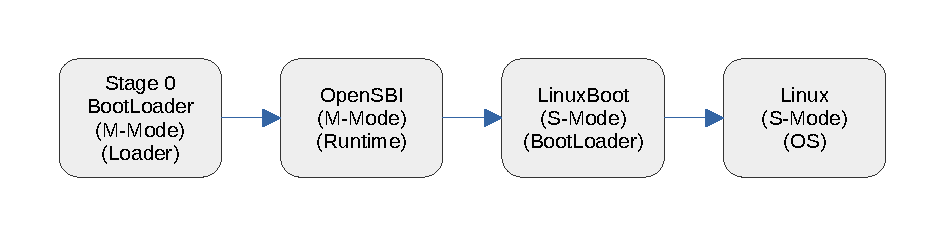
\includegraphics[width=0.9\linewidth]{../images/linux_boot_flow.pdf}
  \caption{Stages of the Linux boot on \textit{RISC-V} on a minimal system.}
  \label{fig:linux_boot_flow}
\end{figure}

\subsection{Open Source Verification tools}
Verification tools are essential when developing hardware or software components. Verification tools allow developers to simulate their work before implementing it in real hardware and test new features in a safe environment where the SoC implementation does not use hardware components. In this thesis project, the author has to simulate hardware logic components and platform-independent software. For that purpose there are three types of verification software that the author is going to use: a \textbf{functional} emulator, a \textbf{cycle-accurate} simulator and an \textbf{event-driven} simulator.

Developers can use cycle-accurate and event-driven simulators to simulate the hardware logic designs. \textbf{Cycle-accurate}  simulators are suitable for complex hardware designs. An example of a cycle-accurate simulator would be \textit{Verilator}. \textbf{Event-driven} simulators are adequate for small hardware designs. An example of an event-driven simulator would be \textit{Icarus Verilog}.

A \textbf{functional} emulator translates the instructions that were supposed to run on the target architecture to instructions that run on the host CPU. The advantage of using a functional emulator is that it is way faster than the other emulation types. An example of a functional emulator would be \textbf{\textit{QEMU}}~\cite{bellard2005qemu}.

\section{Existing Embedded Technologies}
\label{sec:existing_embedded_technologies}
There already exists embedded microcontrollers capable of running Linux. However, most of them are closed source. For example from Arm Holdings (Arm ®), Andes Technology and SiFive. Andes Technology and SiFive are members of the \textit{RISC-V} community and have contributed with open-source components. 

Built upon the \textit{RISC-V} open-source ISA, various open-source CPU designs have emerged. An \textit{application processor} is needed to run a Linux OS. \textit{Application processors} have the necessary CSR, support M+S+U privilege modes, and support atomic instructions. 

An open-source CPU solution would be either the \textit{CVA6}~\cite{zaruba2019cost} (previously known as Ariane), \textit{BOOM}~\cite{zhaosonicboom} or \textit{VexRiscv}~\cite{vexriscv}. The \textit{CVA6} is a 6-stage, single issue, in-order CPU which can execute either the 32-bit or 64-bit \textit{RISC-V} instruction set. The Berkeley Out-of-Order \textit{RISC-V} Processor (\textit{BOOM}) is a superscalar Out-of-Order processor executing the RV64GC variant of the \textit{RISC-V} ISA. The \textit{VexRiscv} CPU is a 32-bit Linux Capable \textit{RISC-V} CPU written in the \textit{SpinalHDL}~\cite{papon2017spinalhdl}.

%%%%%%%%%%%%%%%%%%%%%%%%%%%%%%%%%%%%%%%%%%%%%%%%%%%%%%%%%%%%%%%%%%%%%%
% IMPLEMENTATION
%%%%%%%%%%%%%%%%%%%%%%%%%%%%%%%%%%%%%%%%%%%%%%%%%%%%%%%%%%%%%%%%%%%%%%
%%%%%%%%%%%%%%%%%%%%%%%%%%%%%%%%%%%%%%%%%%%%%%%%%%%%%%%%%%%%%%%%%%%%%%
%     File: ExtendedAbstract_imple.tex                               %
%     Tex Master: ExtendedAbstract.tex                               %
%                                                                    %
%     Author: Andre Calado Marta                                     %
%     Last modified : 27 Dez 2011                                    %
%%%%%%%%%%%%%%%%%%%%%%%%%%%%%%%%%%%%%%%%%%%%%%%%%%%%%%%%%%%%%%%%%%%%%%
% A Calculation section represents a practical development
% from a theoretical basis.
%%%%%%%%%%%%%%%%%%%%%%%%%%%%%%%%%%%%%%%%%%%%%%%%%%%%%%%%%%%%%%%%%%%%%%

\section{IOb-SoC-Linux Hardware Components}
\label{sec:hardware_developed}

The author had to develop four hardware modules to build a SoC capable of executing a Linux OS. Those hardware modules allowed the integration of a new CPU, a new UART and the hardware needed to support interrupts in the \textit{IOb-SoC}. Besides integrating new hardware in the \textit{IOb-SoC}, minor changes to the \textit{IOb-SoC} core were made. The newly used CPU core was generated based on the \textit{SpinalHDL}~\cite{papon2017spinalhdl} \textit{VexRiscv}~\cite{vexriscv} platform. The \textit{VexRiscv} platform enabled the development of a \textit{VexRiscv} CPU core that meets the requirements of an OS. The \textit{VexRiscv} CPU still needed a CPU wrapper to integrate with the \textit{IOb-SoC} interface. The Linux OS also requires a compatible UART to communicate with the user. Linux has drivers that support an existing \textit{UART16550}. A hardware wrapper allows the integration of the \textit{UART16550} on \textit{IOb-SoC-Linux}. Additionally, the SoC has to support timer and software interrupts to run an OS. The CLINT hardware module developed generates timer and software-related interrupts for a \textit{RISC-V} system. Another hardware component which manages interrupts in a \textit{RISC-V} system is the PLIC. A developed hardware component creates an interface with the \textit{IOb-SoC} and instantiates an existing PLIC core and register modules enabling external interrupts on \textit{IOb-SoC-Linux}. 

Figure~\ref{fig:bd_linux} shows a sketch of the SoC developed.

\begin{figure}[!h]
    \centering
    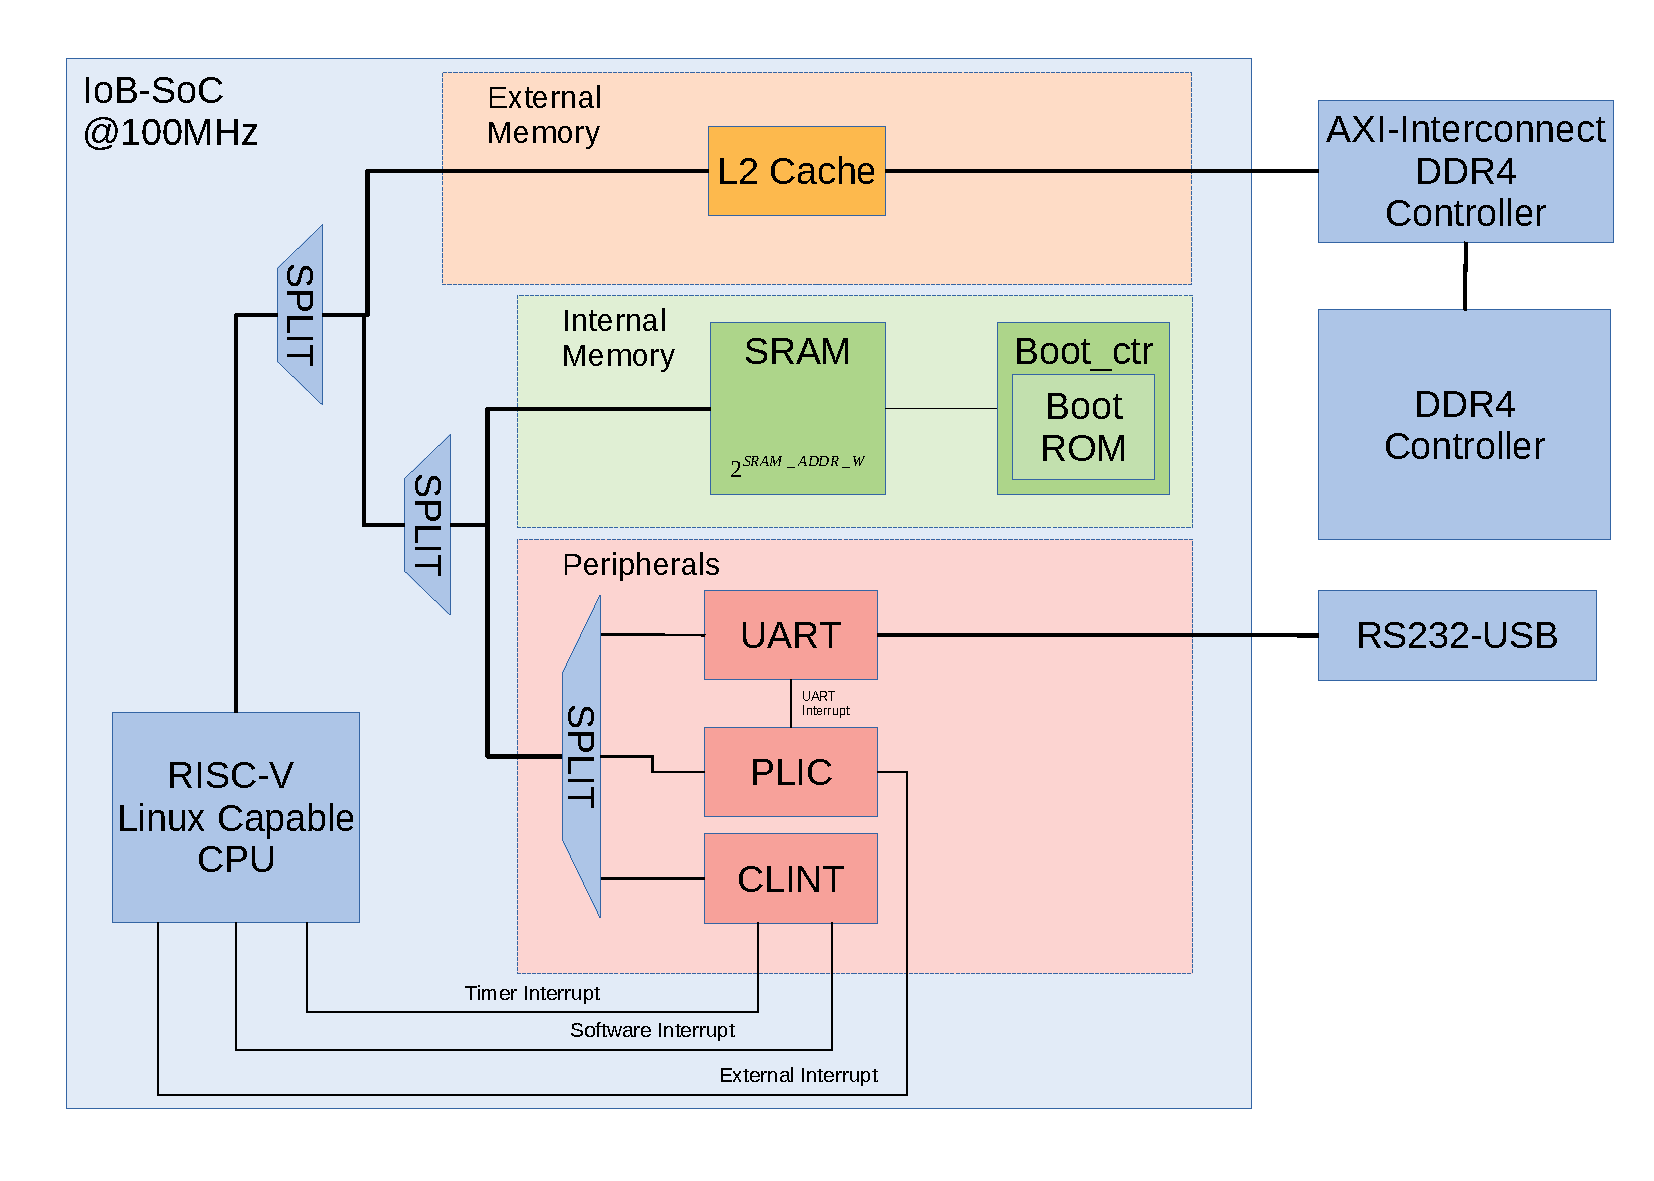
\includegraphics[width=\linewidth]{../images/bd_linux.pdf}
    \caption{Developed SoC sketch.}
    \label{fig:bd_linux}
\end{figure}

\section{Software Components}
\label{sec:software_developed}

During this thesis, the author also developed many software components. Those software components were essential to run a Linux OS in \textit{IOb-SoC} or enhance the \textit{IOb-SoC} platform. First, the new \textit{Console} program written in \textit{Python} allows the \textit{IOb-SoC} platform to communicate through serial with the board. Previously, the \textit{Console} program was written in \textit{C} and had fewer features than the new \textit{Console}. The new \textit{Console} can work with the simulator testbench and communicate with a Linux OS running in \textit{IOb-SoC-Linux}. Secondly, based on the previous \textit{IOb-SoC} verification software, a new hardware simulation testbench can test the SoC and communicate with the \textit{Console} program. Moreover, the \textit{Verilator}~\cite{snyder2010verilator} simulation software allowed the creation of a \textit{Verilator} \textit{C++} testbench to test the SoC faster. Thirdly, a hardware simulation testbench created for the CLINT verifies its behaviour, and a bare-metal interrupt routine firmware developed shows how to use interrupts in \textit{IOb-SoC-Linux}. Finally, the author adapted, built and deployed the software needed to execute a Linux OS in the SoC. The adapted \textit{IOb-SoC} bootloader firmware allows loading the software to the \textit{IOb-SoC-VexRiscv} memory. A device tree file describes the hardware components of the SoC to the Linux kernel. The compiled Linux kernel version must be compatible with the \textit{VexRiscv} CPU, and the root file system developed must be adequate for a minimal Linux OS. While developing the hardware and software components, Makefile scripts helped integrate the components in \textit{IOb-SoC} and automatise the building and deployment process.

Figure \ref{fig:console_flow} presents the \textit{Console} program flowchart.

\begin{figure}[!ht]
    \centering
    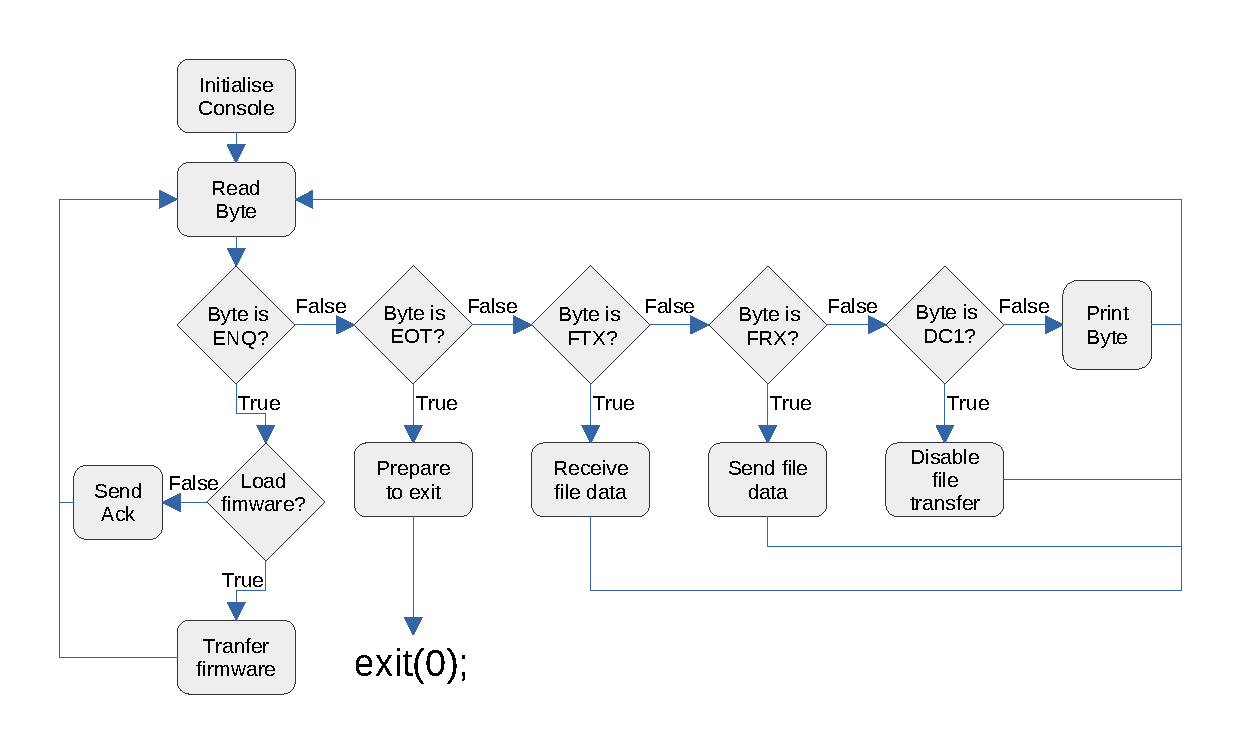
\includegraphics[width=\linewidth]{../images/console_flow.pdf}
    \caption{\textit{Console} program flowchart.}
    \label{fig:console_flow}
\end{figure}

The new verification software interacts with the \textit{Console} through files. Figure~\ref{fig:uut_top_hw} represents a sketch of the verification software and its interaction with the \textit{Console}.

\begin{figure}[!ht]
    \centering
    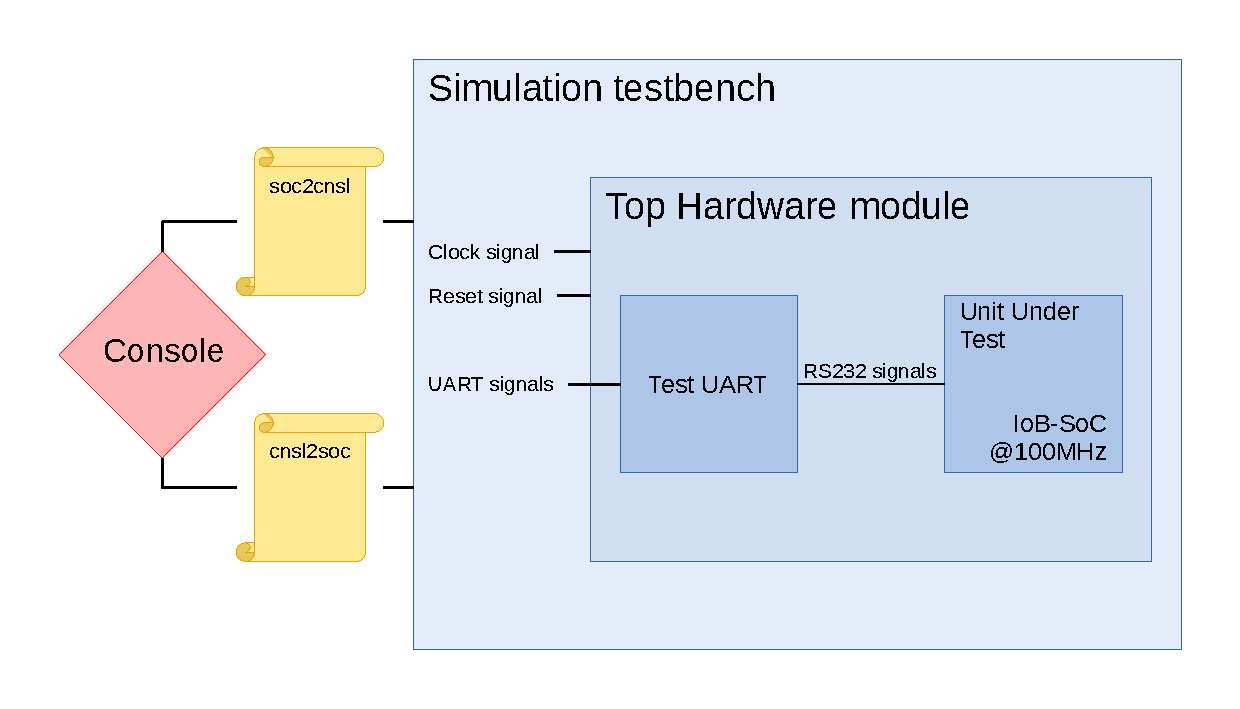
\includegraphics[width=\linewidth]{../images/uut_top_hw.pdf}
    \caption{Simulated hardware interfaces.}
    \label{fig:uut_top_hw}
\end{figure}

%%%%%%%%%%%%%%%%%%%%%%%%%%%%%%%%%%%%%%%%%%%%%%%%%%%%%%%%%%%%%%%%%%%%%%
% RESULTS
%%%%%%%%%%%%%%%%%%%%%%%%%%%%%%%%%%%%%%%%%%%%%%%%%%%%%%%%%%%%%%%%%%%%%%
\section{Project Results}
\label{sec:project_results}
In the following chapter, the author analyses the results obtained from the hardware and software developed in this thesis project. The candidate successfully executes the minimal Linux OS in real hardware using the developed System on a chip. All the results obtained in this thesis which communicate with the FPGA board or the SoC testbench, are executing the developed \textit{Console} program. The hardware components comprising the SoC differ depending on the software needs.

The objective of this thesis project was to run an Operating System in the \textit{IOb-SoC-Linux}. Table \ref{tab:time_os} presents how much time it takes to build the complete OS with the command "make build-OS". The "real" time is the time that passes since the user executes the command until it finishes. The "user" time is the time the CPU takes while executing operations in the user space. The "user" time is bigger than the "real" time because it counts the time passed in each CPU core. Part of the compilation of the RootFS and the kernel is done in parallel using two cores.

\begin{table}[!ht]
    \centering
    \begin{tabular}{ll}
    real & 4m29,570s \\
    user & 8m12,039s \\
    sys  & 0m56,887s
    \end{tabular}
    \caption{Time it takes to build the OS.}
    \label{tab:time_os}
\end{table}

The OS size is to big to run in the FPGA internal memory. The \textit{OpenSBI} bootloader is 90896 Bytes. The device tree blob is 1669 Bytes. The Linux kernel is 4426152 Bytes. Lastly the root file system is 1142733 Bytes. The memory has to have at least 8 MB ($2^23$) to store all this software. However, the Linux kernel needs a bigger memory where it can store virtual memory pages and execute the different application processes. The device tree source describes the system had 512 MB of available memory. Consequently, the author had to implement the \textit{IOb-SoC-Linux} on the FPGA with access to the external memory. The internal memory could never be as big as 512 MB.

In figures \ref{fig:start_bootloader_sim} and \ref{fig:end_bootloader_sim} the reader can see the start of the OS simulation with \textit{Verilator}.

\begin{figure}[!ht]
    \centering
    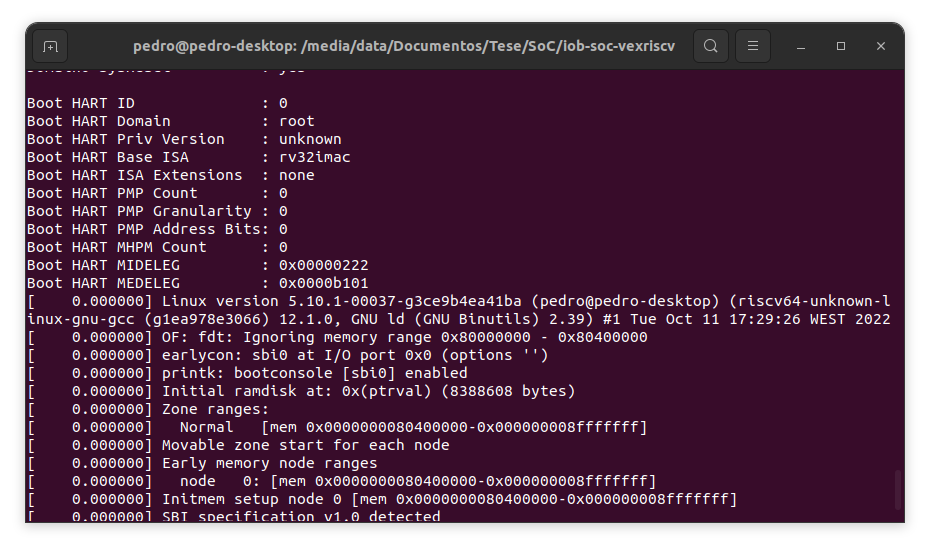
\includegraphics[width=0.5\textwidth]{../images/start_Linux_sim.png}
    \caption{\textit{iob-UART16550} and \textit{iob-PLIC} properties.}
    \label{fig:start_bootloader_sim}
\end{figure}
\begin{figure}[!ht]
    \centering
    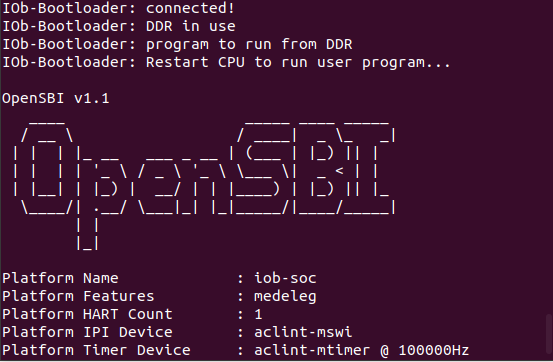
\includegraphics[width=0.5\textwidth]{../images/end_bootloader_sim.png}
    \caption{\textit{IOb-SoC} bootloader and \textit{OpenSBI} firmware.}
    \label{fig:end_bootloader_sim}
\end{figure}

Figure \ref{fig:start_bootloader_sim} shows the initialization of the \textit{Console} program. Furthermore, it shows the instantiation of the \textit{iob-UART16550} and the \textit{iob-PLIC}. The \textit{iob-UART16550} and the PLIC core have an initial block that prints their properties. The synthesis tools do not synthesise the initial block to real hardware, but the simulator executes it. Figure \ref{fig:end_bootloader_sim} shows the \textit{iob-bootloader} and the start of the \textit{OpenSBI} bootloader. The \textit{iob-bootloader} in figure \ref{fig:end_bootloader_sim} does not transfer the software to the memory because the author executed the simulation considering that the software was already in the memory.

Figure \ref{fig:start_linux_sim} shows the end of the \textit{OpenSBI} bootloader and the start of the Linux kernel. The first line printed by the Linux kernel indicates the author built the kernel executing, the kernel version and which toolchain he used to compile it.

\begin{figure}[!ht]
    \centering
    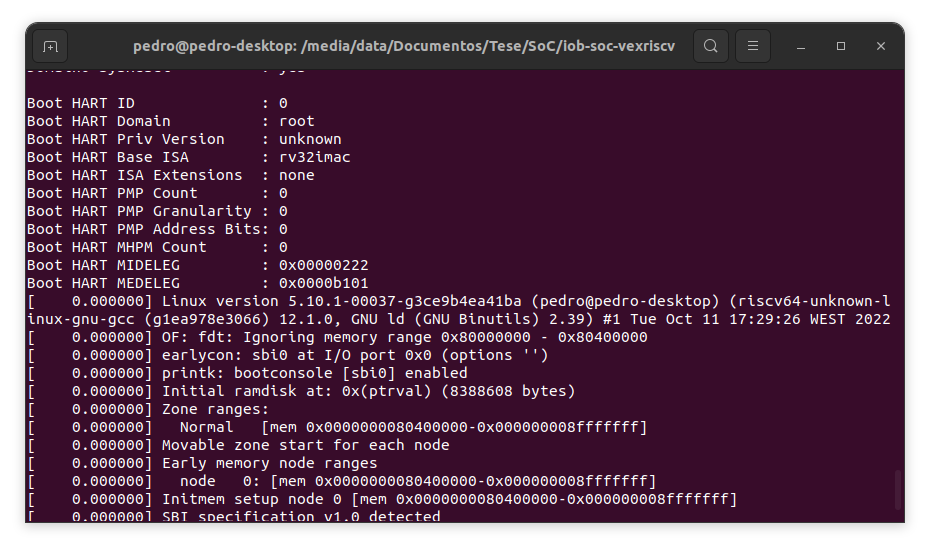
\includegraphics[width=0.5\textwidth]{../images/start_Linux_sim.png}
    \caption{Start of the Linux kernel boot with \textit{Verilator}.}
    \label{fig:start_linux_sim}
\end{figure}

While figure \ref{fig:start_linux_sim} shows the start of the Linux kernel, figure \ref{fig:end_linux_verilator} shows the end of the Linux kernel booting process and the execution of the "init" script. The "init" script is the first program the OS executes after the Linux kernel mounts the RootFS and finishes booting. There exist multiple messages printed to the terminal between the output shown in figure \ref{fig:start_linux_sim} and in \ref{fig:end_linux_verilator}. Those messages show the progress while the Linux kernel boots. The Linux kernel boot process's last message is "Run /init as init process". After that message the SoC executes the "init" program.

\begin{figure}[!ht]
    \centering
    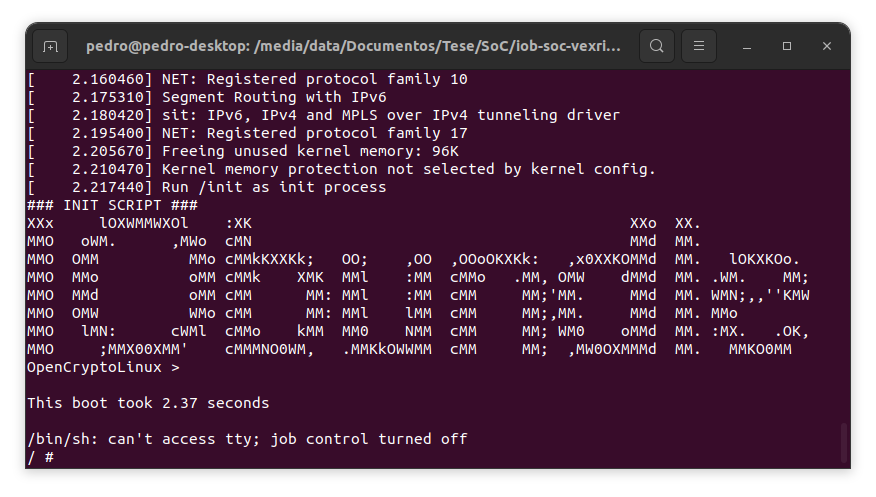
\includegraphics[width=0.5\textwidth]{../images/end_Linux_sim.png}
    \caption{End of Linux kernel boot with \textit{Verilator}.}
    \label{fig:end_linux_verilator}
\end{figure}

Figure \ref{fig:linux_fpga} shows the developed minimal OS running on an FPGA. The reader can see that the author has suppressed the shell warning. The initial part of the figure shows the final stage of the Linux kernel booting. After booting, the author tested the \textit{ls /} command that showed the files and directories in the systems' root. Lastly the author executed the \textit{cat init} command for the OS to print the contents of the "init" script to the terminal.

\begin{figure}[!ht]
    \centering
    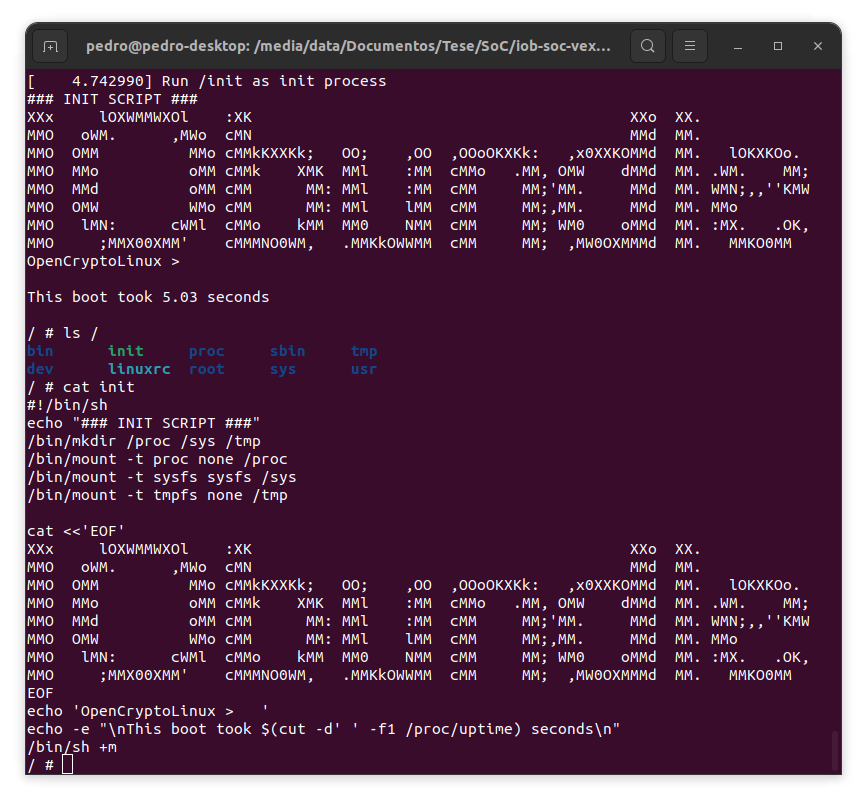
\includegraphics[width=0.5\textwidth]{../images/linux_fpga.png}
    \caption{Linux kernel boot in the FPGA.}
    \label{fig:linux_fpga}
\end{figure}

The time the Linux kernel takes to boot in real hardware, figure \ref{fig:linux_fpga}, is almost double what it takes to boot in simulation, figure \ref{fig:linux_fpga}. The time to boot is almost double because the memory module used in the simulation does not have any latency. When the L2 cache fetches data from memory in real hardware, it must wait before receiving the data burst. Using the \textit{CYCLONE V} FPGA board the Linux kernel takes 7.01 seconds to boot. The author expected the boot to take longer since the system clock frequency used with the \textit{CYCLONE V} is 50 MHz. The Kintex Ultrascale was able to run with a frequency of 100 MHz. The \textit{OpenSBI} bootloader and the device tree blob had to be recompiled with the system frequency defined to 50 MHz to run in the \textit{CYCLONE V}.

A more complex rootfs generated with \textit{Buildroot} provides more features than the minimal rootfs developed. The \textit{Buildroot} rootfs allows using \textit{MicroPython}~\cite{tollervey2017programming} in \textit{IOb-SoC-Linux} and executing the \textit{Dhrystones}~\cite{weicker1984dhrystone} benchmarking software. The rootfs size is a little over 2MB. Figure \ref{fig:linux_buildroot_fpga} shows the final output of the \textit{Dhrystones} benchmark and the execution of simple commands in \textit{MicroPython}. With the \textit{Buildroot} rootfs the Linux kernel takes 6.40 seconds to boot in the \textit{Kintex Ultrascale} and 8.14 seconds in the \textit{CYCLONE V}.

\begin{figure}[!ht]
    \centering
    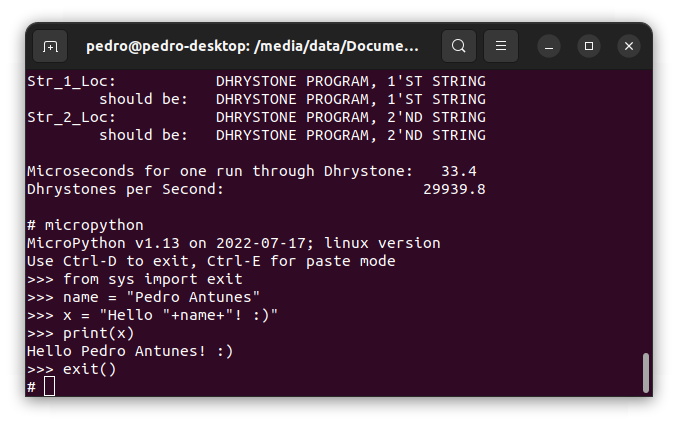
\includegraphics[width=\linewidth]{../images/linux_buildroot_fpga.png}
    \caption{Linux OS with \textit{Buildroot} rootfs.}
    \label{fig:linux_buildroot_fpga}
\end{figure}

\textit{MicroPython} is a software project that aims to implement a \textit{Python} version, highly compatible with \textit{Python3}, in microcontrollers and small embedded systems. \textit{Dhrystones} is a general-performance benchmarking software used in multiple embedded systems. With the \textit{Dhrystones} benchmark, developers can compare the efficiency of different computers or compilers. A common representation of the \textit{Dhrystones} benchmark is \textit{DMIPS}. \textit{DMIPS} is the number of \textit{Dhrystones} per Second divided by 1757, the number of \textit{Dhrystones} per second obtained on the \textit{VAX 11/780}~\cite{emer1984characterization}. Table \ref{tab:dhrystones} represents a comparison between the \textit{Dhrystones} benchmarking scores of both FPGA boards.

\begin{table}[!ht]
    \centering
    \begin{tabular}{l|l|l|}
    \cline{2-3}
                                                         & \textbf{Kintex Ultrascale} & \textbf{CYCLONE V} \\ \hline
    \multicolumn{1}{|l|}{One run through Dhrystone (ms)} & 24.4                       & 33.4               \\ \hline
    \multicolumn{1}{|l|}{Dhrystones per Second}          & 40983.2                    & 29939.8            \\ \hline
    \multicolumn{1}{|l|}{DMIPS}                          & 23.33                      & 17.04            \\ \hline
    \end{tabular}
    \caption{\textit{Dhrystones} benchmarking.}
    \label{tab:dhrystones}
\end{table}

Tables \ref{tab:kintex_linux} and \ref{tab:cyclone_linux} show the resources used by the \textit{IOb-SoC-Linux} in the different FPGAs.

\begin{table}[!ht]
    \centering
    \begin{tabular}{l|l|l|}
        \cline{2-3}
                                            & Resources & FPGA usage \% \\ \hline
        \multicolumn{1}{|l|}{ALM}         & 11,227    & 10                       \\ \hline
        \multicolumn{1}{|l|}{DSP}         & 8         & 3                        \\ \hline
        \multicolumn{1}{|l|}{FF}          & 13725     & 2                        \\ \hline
        \multicolumn{1}{|l|}{BRAM blocks} & 234       & 19                       \\ \hline
        \multicolumn{1}{|l|}{BRAM bits}   & 755,424   & 9                        \\ \hline
    \end{tabular}
    \caption{Cyclone V GT}
    \label{tab:cyclone_linux}
\end{table}
\begin{table}[!ht]
    \centering
    \begin{tabular}{l|l|l|}
        \cline{2-3}
                                        & Resources & FPGA usage \% \\ \hline
        \multicolumn{1}{|l|}{LUTs}      & 23126     & 9.54                     \\ \hline
        \multicolumn{1}{|l|}{Registers} & 24505     & 5.05                     \\ \hline
        \multicolumn{1}{|l|}{DSPs}      & 10        & 0.52                     \\ \hline
        \multicolumn{1}{|l|}{BRAM}      & 39.5      & 6.58                     \\ \hline
    \end{tabular}
    \caption{Kintex Ultrascale}
    \label{tab:kintex_linux}
\end{table}

Tables \ref{tab:kintex_linux} and \ref{tab:cyclone_linux} show that the resources utilization from the \textit{IOb-SoC-Linux} is not much bigger than the \textit{IOb-SoC}. The FPGA still has enough resources to implement hardware accelerators.


%%%%%%%%%%%%%%%%%%%%%%%%%%%%%%%%%%%%%%%%%%%%%%%%%%%%%%%%%%%%%%%%%%%%%%
% CONCLUSIONS
%%%%%%%%%%%%%%%%%%%%%%%%%%%%%%%%%%%%%%%%%%%%%%%%%%%%%%%%%%%%%%%%%%%%%%
%%%%%%%%%%%%%%%%%%%%%%%%%%%%%%%%%%%%%%%%%%%%%%%%%%%%%%%%%%%%%%%%%%%%%%
%     File: ExtendedAbstract_concl.tex                               %
%     Tex Master: ExtendedAbstract.tex                               %
%                                                                    %
%     Author: Andre Calado Marta                                     %
%     Last modified : 27 Dez 2011                                    %
%%%%%%%%%%%%%%%%%%%%%%%%%%%%%%%%%%%%%%%%%%%%%%%%%%%%%%%%%%%%%%%%%%%%%%
% The main conclusions of the study presented in short form.
%%%%%%%%%%%%%%%%%%%%%%%%%%%%%%%%%%%%%%%%%%%%%%%%%%%%%%%%%%%%%%%%%%%%%%

\section{Conclusions}
\label{sec:concl}

Conclusions, future work and some final remarks...



%%%%%%%%%%%%%%%%%%%%%%%%%%%%%%%%%%%%%%%%%%%%%%%%%%%%%%%%%%%%%%%%%%%%%%
% ACKNOWLEDGMENTS
%%%%%%%%%%%%%%%%%%%%%%%%%%%%%%%%%%%%%%%%%%%%%%%%%%%%%%%%%%%%%%%%%%%%%%
%%%%%%%%%%%%%%%%%%%%%%%%%%%%%%%%%%%%%%%%%%%%%%%%%%%%%%%%%%%%%%%%%%%%%%
%     File: ExtendedAbstract_ackno.tex                               %
%     Tex Master: ExtendedAbstract.tex                               %
%                                                                    %
%     Author: Andre Calado Marta                                     %
%     Last modified : 27 Dez 2011                                    %
%%%%%%%%%%%%%%%%%%%%%%%%%%%%%%%%%%%%%%%%%%%%%%%%%%%%%%%%%%%%%%%%%%%%%%
% Acknowledge persons and institutions that supported this work.
%%%%%%%%%%%%%%%%%%%%%%%%%%%%%%%%%%%%%%%%%%%%%%%%%%%%%%%%%%%%%%%%%%%%%%

\section*{Acknowledgements}

The author would like to thank his friends and professors who helped and accompanied him through his studies. Furthermore, above all, the author is thankful for his family that has been in his life since day 0, giving advice and guiding him, leading him to where he is today.



%%%%%%%%%%%%%%%%%%%%%%%%%%%%%%%%%%%%%%%%%%%%%%%%%%%%%%%%%%%%%%%%%%%%%%
% REFERENCES
%%%%%%%%%%%%%%%%%%%%%%%%%%%%%%%%%%%%%%%%%%%%%%%%%%%%%%%%%%%%%%%%%%%%%%

% Produces the bibliography section when processed by BibTeX
%
% Bibliography style
% > entries ordered alphabetically
%\bibliographystyle{plain}
% > unsorted with entries appearing in the order in which the citations appear.
%\bibliographystyle{unsrt}
% > entries ordered alphabetically, with first names and names of journals and months abbreviated
\bibliographystyle{abbrv}
% > entries ordered alphabetically, with reference markers based on authors' initials and publication year
%\bibliographystyle{alpha}

% External bibliography database file in the BibTeX format (ExtendedAbstract_ref_db.bib)
\bibliography{ExtendedAbstract_ref_db}

%%%%%%%%%%%%%%%%%%%%%%%%%%%%%%%%%%%%%%%%%%%%%%%%%%%%%%%%%%%%%%%%%%%%%%
\end{document}
%%%%%%%%%%%%%%%%%%%%%%%%%%%%%%%%%%%%%%%%%%%%%%%%%%%%%%%%%%%%%%%%%%%%%%

